\documentclass[12pt, oneside]{article}

\usepackage[letterpaper, scale=0.89, centering]{geometry}
\usepackage{fancyhdr}
\setlength{\parindent}{0em}
\setlength{\parskip}{1em}

\usepackage{tikz}
\usetikzlibrary{automata,positioning,arrows}

\pagestyle{fancy}
\fancyhf{}
\renewcommand{\headrulewidth}{0pt}
\rfoot{\href{https://creativecommons.org/licenses/by-nc-sa/2.0/}{CC BY-NC-SA 2.0} Version \today~(\thepage)}

\usepackage{amssymb,amsmath,pifont,amsfonts,comment,enumerate,enumitem}
\usepackage{currfile,xstring,hyperref,tabularx,graphicx,wasysym}
\usepackage[labelformat=empty]{caption}
\usepackage{xcolor}
\usepackage{multicol,multirow,array,listings,tabularx,lastpage,textcomp,booktabs}

% NOTE(joe): This environment is credit @pnpo (https://tex.stackexchange.com/a/218450)
\lstnewenvironment{algorithm}[1][] %defines the algorithm listing environment
{   
    \lstset{ %this is the stype
        mathescape=true,
        frame=tB,
        numbers=left, 
        numberstyle=\tiny,
        basicstyle=\rmfamily\scriptsize, 
        keywordstyle=\color{black}\bfseries,
        keywords={,procedure, div, for, to, input, output, return, datatype, function, in, if, else, foreach, while, begin, end, }
        numbers=left,
        xleftmargin=.04\textwidth,
        #1
    }
}
{}

\newcommand\abs[1]{\lvert~#1~\rvert}
\newcommand{\st}{\mid}

\newcommand{\cmark}{\ding{51}}
\newcommand{\xmark}{\ding{55}}


\begin{document}
\begin{flushright}
    \StrBefore{\currfilename}{.}
\end{flushright}

\section*{Before we start}

We are committed to fostering a learning environment for this course that supports a diversity of thoughts, 
perspectives and experiences, and respects your identities (including race, ethnicity, heritage, gender, sex, 
class, sexuality, religion, ability, age, educational background, etc.).  
Our goal is to create a diverse and inclusive learning environment where all students feel comfortable and can thrive. 

If you or someone you know is suffering from food and/or housing insecurities 
there are UCSD resources here to help:

Basic Needs Office: \href{https://basicneeds.ucsd.edu/}{https://basicneeds.ucsd.edu/}

Triton Food Pantry (in the old Student Center)
is free and anonymous, and includes produce: 

\href{https://www.facebook.com/tritonfoodpantry/}{https://www.facebook.com/tritonfoodpantry/}

Mutual Aid UCSD: \href{https://mutualaiducsd.wordpress.com/}{https://mutualaiducsd.wordpress.com/}

Financial aid resources, the possibility of emergency grant funding, and off-campus housing referral 
resources are available. See CAPS and your college dean.

If you find yourself in an uncomfortable situation, ask for help. 
We are committed to upholding University policies regarding nondiscrimination, sexual violence and sexual harassment.

Counseling and Psychological Services (CAPS) at 858 5343755 or \href{http://caps.ucsd.edu}{http://caps.ucsd.edu}


OPHD at (858) 534-8298, ophd@ucsd.edu , \href{http://ophd.ucsd.edu}{http://ophd.ucsd.edu}. 
CARE at Sexual Assault Resource Center at 858 5345793 sarc@ucsd.edu \href{http://care.ucsd.edu}{http://care.ucsd.edu}


Please do not come to class if you are sick or even think you might be sick.
We will continue to follow the campus guidelines as updated on https://returntolearn.ucsd.edu/ .

Please reach out (minnes@ucsd.edu or dgrier@ucsd.edu) if you need support with extenuating circumstances.

\newpage

\section*{Introductions}
Class website: \href{https://canvas.ucsd.edu/courses/45073}{https://canvas.ucsd.edu/courses/45073}


Instructor for A00: Prof. Mia Minnes {\tiny{"Minnes" rhymes with Guinness}}, minnes@ucsd.edu, 
\href{http://cseweb.ucsd.edu/~minnes}{http://cseweb.ucsd.edu/~minnes}

Instructor for B00: Prof. Daniel Grier, dgrier@ucsd.edu, \href{http://danielgrier.com/}{http://danielgrier.com/}

Our team: Two instructors + four TAs and nine tutors + all of you

Fill in contact info for students around you, if you'd like:

\vfill


On a typical week: {\bf MWF} Lectures + review quizzes, {\bf Tu} Homework due, {\bf WF} Discussion.
Office hours (hosted by instructors and TAs and tutors, where you can come to talk 
about course concepts and ask for help as you work through sample problems) and Q+A on Piazza available throughout the week.
All dates are on \href{https://canvas.ucsd.edu/}{Canvas (click for link)} and details are on
 \href{https://canvas.ucsd.edu/courses/45073}{the Syllabus page}.

\newpage Welcome to CSE 105: Introduction to Theory of Computation in Winter 2024!

\section*{CSE 105's Big Questions}
\begin{itemize}
   \item What problems are computers capable of solving?
   \item What resources are needed to solve a problem?
   \item Are some problems harder than others?
\end{itemize}

In this context, a {\bf problem} is defined as: ``Making a decision or computing a value based on some input"

Consider the following problems: 
\begin{itemize}
   \item Find a file on your computer
   \item Determine if your code will compile
   \item Find a run-time error in your code
   \item Certify that your system is un-hackable
\end{itemize}

Which of these is hardest?

\vfill

In Computer Science, we operationalize ``hardest'' as ``requires most resources'', where
resources might be memory, time, parallelism, randomness, power, etc.

To be able to compare ``hardness'' of problems, we use a consistent description of problems

{\bf Input}: String

{\bf Output}: Yes/ No, where Yes means that the input string matches the pattern or property described by the problem.


\newpage
\section*{Monday}

%! app: Regular Languages
%! outcome: Define decision problem

The CSE 105 vocabulary and notation build on discrete
math and introduction to proofs classes.  Some of the conventions may 
be a bit different so we'll draw your attention to them.

For consistency, we will use the notation from this class' textbook\footnote{Page references are to 
the 3rd edition (International) of Sipser's Introduction to the Theory of Computation,
available through various sources for under \$30. You may be able to 
opt in to purchase a digital copy through Canvas. Copies of the book are also available 
for those who can't access the book
to borrow from the course instructor, while supplies last (minnes@ucsd.edu)}.

These definitions are on pages 3, 4, 6, 13, 14, 53.

\begin{center}
    \begin{tabular}{|p{2.6in}cp{3.5in}|}
    \hline 
    {\bf Term} & {\bf Typical symbol} & {\bf Meaning} \\
     & or {\bf Notation} & \\
    \hline
    && \\
    Alphabet & $\Sigma$, $\Gamma$ & A non-empty finite set	 \\
    Symbol over $\Sigma$  & $\sigma$, $b$, $x$ & An element of the alphabet $\Sigma$\\ 
    String over $\Sigma$  &	$u$, $v$, $w$ & A finite list of symbols from $\Sigma$\\
    (The) empty string &$\varepsilon$ & The (only) string of length $0$\\
    The set of all strings over $\Sigma$ & $\Sigma^*$ & The collection of all possible strings formed from symbols from $\Sigma$ \\ 
    (Some) language over $\Sigma$& $L$ & (Some) set of strings over $\Sigma$ \\ 
    (The) empty language &$\emptyset$ & The empty set, i.e. the set that has no strings (and no other elements either)\\
    && \\
    \hline
    && \\
    The power set of a set $X$ &$\mathcal{P}(X)$ & The set of all subsets of $X$ \\
    (The set of) natural numbers &$\mathcal{N}$ & The set of positive integers \\ 
    (Some) finite set & & The empty set or a set whose distinct elements can be counted by a natural number\\
    (Some) infinite set & & A set that is not finite.\\ 
    &&\\
    \hline
    && \\
    Reverse of a string $w$ & $w^\mathcal{R}$  & write $w$  in  the opposite order, if $w = w_1 \cdots  w_n$ then $w^\mathcal{R} = w_n \cdots  w_1$. Note: $\varepsilon^\mathcal{R} = \varepsilon$\\
    Concatenating strings $x$ and $y$ & $xy$ &  take $x = x_1 \cdots x_m$, $y=y_1 \cdots y_n$ and form $xy = x_1 \cdots x_m y_1 \cdots y_n$\\
    String $z$ is a substring of string $w$ & & there are strings $u,v$ such that $w = uzv$\\
    String $x$ is a prefix of string $y$ & & there is a string $z$ such that $y = xz$ \\
    String $x$ is a proper prefix of string $y$ & & $x$ is a prefix of $y$ and $x \neq y$\\
    && \\
    \hline
    &&\\
    Shortlex order, also known as string order over alphabet $\Sigma$ & & Order strings over  $\Sigma$ first by length and then according to the dictionary order, assuming symbols in $\Sigma$  have an ordering.\\ \hline
    \end{tabular}
\end{center}

\vfill
    

Write out in words the meaning of the symbols below: 
\[
    \{ a,b, c\}
\]

\phantom{The set whose elements are $a$, $b$, and $c$}

\[
    | \{a, b, a \} | = 2
\]

\phantom{The number of elements in the set $\{a,b,a\}$ is $2$.}

\[
    | aba | = 3
\]

\phantom{The length of the string $aba$ is $3$.}

\[
    (a, 3, 2, b, b)
\]

\phantom{The $5$-tuple whose first components is $a$, second component 
is $3$, third component is $2$, fourth component is $b$, and fifth component is $b$.}


{\it Circle the correct choice}:

A {\bf string} over an alphabet $\Sigma$ is \underline{~~an element of $\Sigma^*$ ~~ OR ~~ a subset of $\Sigma^*$}.
    
A {\bf language} over an alphabet $\Sigma$ is \underline{~~an element of $\Sigma^*$ ~~ OR ~~ a subset of $\Sigma^*$}.


{\it Extra examples for practice:}

With $\Sigma_1 = \{0,1\}$ and $\Sigma_2 = \{a,b,c,d,e,f,g,h,i,j,k,l,m,n,o,p,q,r,s,t,u,v,w,x,y,z\}$  and $\Gamma = \{0,1,x,y,z\}$

An example of a string of length 3 over $\Sigma_1$ is \underline{\phantom{ $000$} \hspace{0.2in}}

An example of  a string of length 1 over $\Sigma_2$ is  \underline{\phantom{ $k$} \hspace{0.2in}}

The number of distinct strings of length 2 over $\Gamma$ is  \underline{\phantom{ $25$} \hspace{0.2in}}

An example of a language over $\Sigma_1$ of size $1$ is  \underline{\phantom{ $ \{ \varepsilon \} $} \hspace{0.2in}}

An example of an infinite language over $\Sigma_1$ is  \underline{\phantom{ $\Sigma^*$} \hspace{0.2in}}
    
An example of  a finite language over $\Gamma$ is  \underline{\phantom{ $\{ 0, x \}$} \hspace{0.2in}}
    
{\bf True} or {\bf False}: $\varepsilon \in \Sigma_1$

{\bf True} or {\bf False}: $\varepsilon$ is  a string over $\Sigma_1$

{\bf True} or {\bf False}: $\varepsilon$ is a language over $\Sigma_1$

{\bf True} or {\bf False}: $\varepsilon$ is a prefix of some string over  $\Sigma_1$

{\bf True} or {\bf False}: There is a string over $\Sigma_1$ that is a proper prefix of $\varepsilon$
    

The first five strings over $\Sigma_1$ in string order, using the ordering $0 <  1$: \vfill
    
The first five strings over $\Sigma_2$ in string order, using the usual alphabetical ordering for single letters: \vfill

    
\newpage
\subsection*{Review: Week 1 Monday}
\begin{enumerate}
\item Please complete the beginning of the quarter survey linked from our \#FinAid
Assignment on Canvas \href{https://canvas.ucsd.edu/courses/45073/assignments/609253}{https://canvas.ucsd.edu/courses/45073/assignments/609253?wrap=1}
\item We want you to be familiar with class policies and procedures so you are ready to have a successful quarter. 
Please take a look at the syllabus on our class website https://canvas.ucsd.edu/courses/45073
and answer the questions about it on Gradescope.
\end{enumerate}

A summary of the terminology we will use is on page 16 in the textbook.

{\bf Pre class reading for next time}: Example 1.51, Definition 1.52

{\it Notice}: we are jumping to Section 1.3 Regular Expressions and then will come back 
to Section 1.1 Finite Automata on Friday.


\newpage
\subsection*{Week 1 Wednesday}

%! app: Regular Languages
%! outcome: Regular expressions

Our motivation in studying sets of strings is that they can be used to encode problems.
To calibrate how difficult a problem is to solve, we describe how complicated the set of strings that encodes it is. 
How do we define sets of strings?


\vfill

How would you describe the language that has no elements at all?

\vfill

How would you describe the language that has all strings over $\{0,1\}$ as its elements?

\vfill

\newpage

**This definition was in the pre-class reading**
{\bf Definition 1.52}: A {\bf regular expression} over alphabet $\Sigma$
is a syntactic expression that can describe a language over $\Sigma$. The collection of all regular
expressions over $\Sigma$ is defined recursively:
\begin{itemize}
\item[] {\it Basis steps of recursive definition}
\begin{quote}    
    $a$ is a regular expression, for $a \in \Sigma$

    $\varepsilon$ is a regular expression

    $\emptyset$ is a regular expression
\end{quote}

\item[] {\it Recursive steps of recursive definition}
\begin{quote}
    $(R_1 \cup R_2)$ is a regular expression when $R_1$, $R_2$ are regular expressions 

    $(R_1 \circ R_2)$ is a regular expression when $R_1$, $R_2$ are regular expressions

    $(R_1^*)$ is a regular expression when $R_1$ is a regular expression 
\end{quote}
\end{itemize}
 

The {\it semantics} (or meaning) of the syntactic regular expression is the {\bf language
described by the regular expression}. The function that assigns a language to a regular expression
over $\Sigma$ is defined recursively, using familiar set operations:


\begin{itemize}
    \item[] {\it Basis steps of recursive definition}
    \begin{quote}    
        The language described by $a$, for $a \in \Sigma$, is $\{a\}$ and we write 
        $L(a) = \{a\}$
    
        The language described by $\varepsilon$ is $\{\varepsilon\}$ and we write 
        $L(\varepsilon) = \{ \varepsilon\}$
    
        The language described by $\emptyset$ is $\{\}$ and we write
        $L(\emptyset) = \emptyset$.
    \end{quote}
    
    \item[] {\it Recursive steps of recursive definition}
    \begin{quote}
        When $R_1$, $R_2$ are regular expressions, the language described by the regular
        expression $(R_1 \cup R_2)$ is the union of the languages described by $R_1$ and $R_2$, 
        and we write 
        $$L(~(R_1 \cup R_2)~) = L(R_1) \cup L(R_2) = \{ w \mid w \in L(R_1) \lor w \in L(R_2)\}$$
    
        When $R_1$, $R_2$ are regular expressions, the language described by the regular
        expression $(R_1 \circ R_2)$ is the concatenation of the languages described by $R_1$ and $R_2$, 
        and we write 
        $$L(~(R_1 \circ R_2)~) = L(R_1) \circ L(R_2) = \{ uv \mid u \in L(R_1) \land v \in L(R_2)\}$$
    
        When $R_1$ is a regular expression, the language described by the regular 
        expression $(R_1^*)$ is the {\bf Kleene star} of the language described by $R_1$ and we write
        $$L(~(R_1^*)~) = (~L(R_1)~)^* = \{ w_1 \cdots w_k \mid k \geq 0 \textrm{ and each } w_i \in L(R_1)\}$$
    \end{quote}
\end{itemize}
  
\newpage
For the following examples assume the alphabet is $\Sigma_1 =  \{0,1\}$:
    
The language described by the regular expression $0$ is $L(0) = \{ 0 \}$

The language described by the regular expression $1$ is $L(1)  = \{ 1 \}$

The language described by the regular expression $\varepsilon$ is $L(\varepsilon) = \{ \varepsilon  \}$

The language described by the regular expression $\emptyset$ is $L(\emptyset) = \emptyset$

The language described by the regular expression $(\Sigma_1 \Sigma_1 \Sigma_1)^*$ 
is $L(~(\Sigma_1 \Sigma_1 \Sigma_1)^*~) = $

\vfill

The language described by the regular expression $1^+$ is $L(~(1^+)~) = L(1^* \circ 1) = $

\vfill


{\it Shorthand and conventions} (Sipser pages 63-65)
\begin{center}
    \begin{tabular}{|ll|}
    \hline
    & \\
    \multicolumn{2}{|l|}{Assuming $\Sigma$ is the alphabet, we use the following conventions}\\
    & \\
    $\Sigma$   & regular  expression describing language consisting of  all strings  of length  $1$ over $\Sigma$\\
    $*$ then $\circ$ then $\cup$   & precedence order, unless parentheses are used to change it\\
    $R_1R_2$ & shorthand  for  $R_1  \circ R_2$ (concatenation symbol is implicit) \\
    $R^+$ & shorthand for $R^* \circ R$ \\
    $R^k$ & shorthand for $R$ concatenated with itself $k$ times, where $k$ is a (specific) natural number\\
    & \\
    \hline
    \end{tabular}
\end{center}

\newpage
{\bf Caution: many programming languages that support regular expressions build in functionality
that is more powerful than the ``pure'' definition of regular expressions given here. }

Regular expressions are everywhere (once you start looking for them).

Software tools and languages often have built-in support for regular expressions to describe
{\bf patterns} that we want to match (e.g. Excel/ Sheets, grep, Perl, python, Java, Ruby).

Under the hood, the first phase of {\bf compilers} is to transform the strings we write 
in code to tokens (keywords, operators, identifiers, literals). Compilers use regular expressions
to describe the sets of strings that can be used for each token type.

Next time: we'll start to see how to build machines that decide whether strings match the pattern
described by a regular expression.

\vfill


{\it Extra examples for practice:}

Which regular expression(s) below describe a language that includes the string $a$ as an element?

$a^* b^*$ 

\vfill

$a(ba)^* b$

\vfill

$a^* \cup b^*$

\vfill

$(aaa)^*$

\vfill

$(\varepsilon \cup a) b$

\vfill

\newpage
\subsection*{Review: Week 1 Wednesday}

Please complete the review quiz questions on \href{http://gradescope.com}{Gradescope} about 
strings, languages, and regular expressions.


Recall: Review quizzes based on class material are assigned each day. 
These quizzes will help you track and confirm your understanding of the concepts and examples 
we work in class. Quizzes can be submitted on Gradescope as many times (with no penalty) as 
you like until the quiz deadline: the three quizzes each week are all due on Friday (with no penalty 
late submission open until Sunday).

The definition of the union, concatenation, and star operations for languages is given 
as Definition 1.23 on page 44 and a useful example is Example 1.24.

{\bf Pre class reading for next time}: Figure 1.4, Definition 1.5

{\it Notice}: On Friday we are going back to the start of Chapter 1 and will be discussing finite 
automata and their computations.

\newpage
\subsection*{Week 1 Friday}

%! app: regular-languages
%! outcome: Regular expressions, Formal definition of automata, Informal definition of automata

{\bf Review}: Determine whether each statement below about regular expressions
over the alphabet $\{a,b,c\}$ is true or false:
   
True or False: \qquad 
   $a  \in L(~(a \cup b )~\cup c)$

True or False: \qquad 
   $ab  \in L(~ (a \cup b)^*  ~)$
   
True or False: \qquad    
   $ba \in L( ~ a^* b^* ~)$
   
True or False: \qquad 
   $\varepsilon  \in L(a \cup b \cup c)$
   
True or False: \qquad 
   $\varepsilon  \in L(~ (a \cup b)^*  ~)$

True or False: \qquad 
   $\varepsilon \in L( ~ a^* b^* ~)$


{\bf From the pre-class reading, pages 34-36}:
A deterministic finite automaton (DFA) is specified by  $M = (Q, \Sigma, \delta, q_0, F)$.
This $5$-tuple is called the {\bf formal definition} of the DFA. The DFA can also 
be represented by its state diagram: with nodes for the state, labelled edges specifying the 
transition function, and decorations on nodes denoting the start and accept states.

\begin{quote}
Finite set of states $Q$ can be labelled by any collection of distinct names. Often
we use default state labels $q0, q1, \ldots$ 
\end{quote}

\begin{quote}  
The alphabet $\Sigma$ determines the possible inputs to the automaton. 
Each input to the automaton is a string over  $\Sigma$, and the automaton ``processes'' the input
one symbol (or character) at a time.
\end{quote}

\begin{quote}
The transition function $\delta$ gives the next state of the DFA based on the current state of 
the machine and on the next input symbol.
\end{quote}

\begin{quote}
The start state $q_0$ is an element of $Q$.  Each computation of the machine starts at the  start  state.
\end{quote}

\begin{quote}
The accept (final) states $F$ form a subset of the states of the DFA, $F \subseteq  Q$. 
These states are used to flag if the machine accepts or rejects an input string.
\end{quote}


\begin{quote}
The computation of a machine on an input string is a sequence of states
in the machine,  starting with the start state, determined by transitions 
of the machine as it reads successive input symbols.
\end{quote}

\begin{quote}
The DFA $M$ accepts the given input string exactly when the computation of $M$ on the input string
ends in an accept state. $M$ rejects the given input string exactly when the computation of 
$M$ on the input string ends in a nonaccept state, that is, a state that is not in $F$.
\end{quote}

\begin{quote} 
The language of $M$, $L(M)$, is defined as the set of  all strings that are each accepted 
by the machine $M$. Each string that is rejected by $M$ is not in $L(M)$.
The language of $M$ is also called the language recognized by $M$.
\end{quote}   
   
What is {\bf finite} about all deterministic finite automata? (Select all that apply)
\begin{itemize}
   \item[$\square$] The size of the machine (number of states, number of arrows)
   \item[$\square$] The number of strings that are accepted by the machine
   \item[$\square$] The length of each computation of the machine
\end{itemize}
  
\begin{figure}[h]
   \centering
   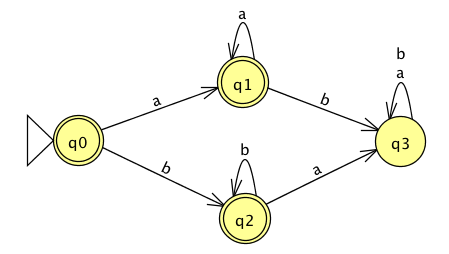
\includegraphics[width=3in]{../../resources/machines/Lect2DFA1.png} 
\end{figure}
   
The formal definition of this DFA is
   
\vspace{100pt}
   

Classify each string $a, aa, ab, ba, bb, \varepsilon$ as accepted by the DFA or rejected by the DFA.  

{\it Why are these the only two options?}

\vspace{200pt}


The language recognized by this DFA is
  
\vspace{100pt}
   

\begin{figure}[h]
  \centering
  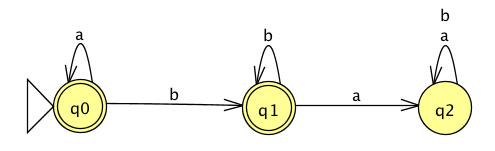
\includegraphics[width=3in]{../../resources/machines/Lect2DFA2.png} 
\end{figure}
   

The language recognized by this DFA is
  
\vspace{100pt}

\begin{figure}[h]
    \centering
    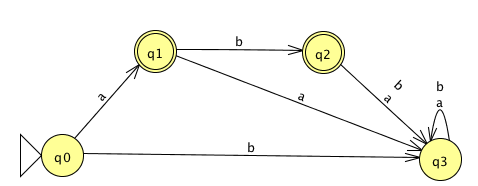
\includegraphics[width=3in]{../../resources/machines/Lect2DFA3.png} 
\end{figure}

The language recognized by this DFA is
  
\vspace{100pt}



\newpage

\subsection*{Review: Week 1 Friday}

Please complete the review quiz questions on \href{http://gradescope.com}{Gradescope} about 
DFA and the strings they accept and reject.

The definition of the union, concatenation, and star operations for languages is given 
as Definition 1.23 on page 44 and a useful example is Example 1.24.


The first homework assignment for CSE 105 this quarter is due next week. 
Find it on the class website: in the Calendar section of the website, click on the link under "Due Dates" for Week 2, or find
the detailed assignment in the Assignments section of the website.
Due: 4/11/23 at 5pm (no penalty late submission until 8am next morning)

We encourage you to work on homework in groups of up to three CSE 105 classmates. 
To find group members: reach out to people sitting around you in class, in discussion section, 
or during office hours. The pre-survey also asks if you want help finding group members: 
the CSE 105 instructional team can help you connect with other students. Working within the 
campus safety guidelines, you may choose to meet with your group mates in person or remotely. 
We highly recommend meeting synchronously so that you can work through the homework problems *together*. 

{\bf Pre class reading for next time}: pages 41-43 (figures 1.18, 1.19, 1.20)

\end{document}